\documentclass{standalone}
\usepackage{tikz}
\usetikzlibrary{patterns, positioning}

\begin{document}
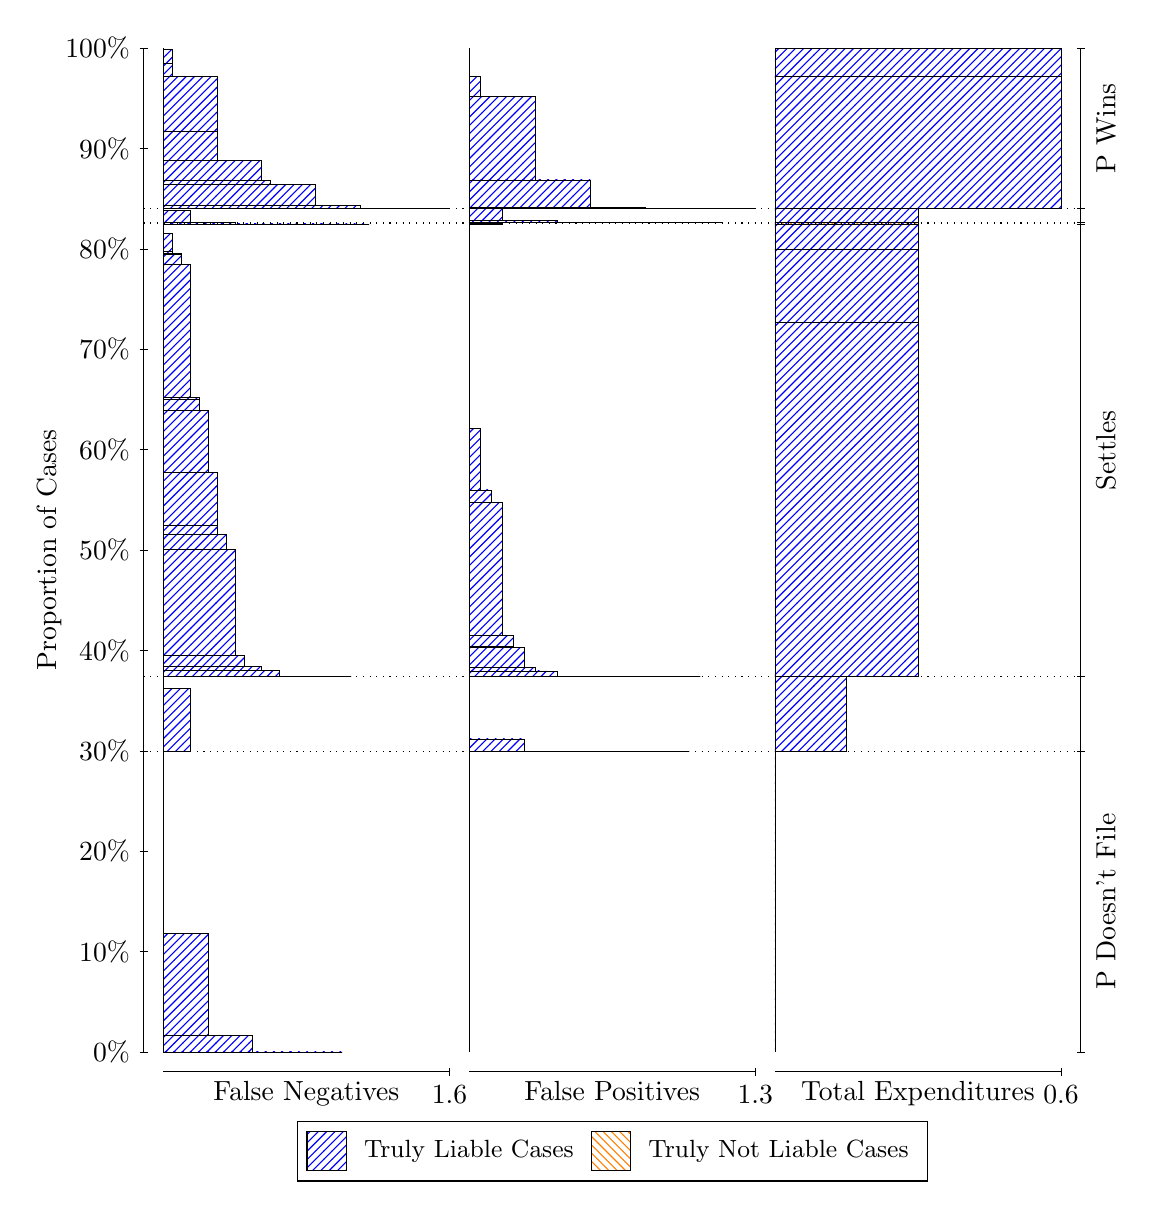
\begin{tikzpicture}
\draw[black, very thin] (1.5,1.75) -- (1.5,14.5);
\node[rotate=90, anchor=center] at (0.3, 8.125) {Proportion of Cases};
\draw[black, very thin] (1.45,1.75) -- (1.55,1.75);
\node[anchor=east] at (1.45, 1.75) {0\%};
\draw[black, very thin] (1.45,3.025) -- (1.55,3.025);
\node[anchor=east] at (1.45, 3.025) {10\%};
\draw[black, very thin] (1.45,4.3) -- (1.55,4.3);
\node[anchor=east] at (1.45, 4.3) {20\%};
\draw[black, very thin] (1.45,5.575) -- (1.55,5.575);
\node[anchor=east] at (1.45, 5.575) {30\%};
\draw[black, very thin] (1.45,6.85) -- (1.55,6.85);
\node[anchor=east] at (1.45, 6.85) {40\%};
\draw[black, very thin] (1.45,8.125) -- (1.55,8.125);
\node[anchor=east] at (1.45, 8.125) {50\%};
\draw[black, very thin] (1.45,9.4) -- (1.55,9.4);
\node[anchor=east] at (1.45, 9.4) {60\%};
\draw[black, very thin] (1.45,10.675) -- (1.55,10.675);
\node[anchor=east] at (1.45, 10.675) {70\%};
\draw[black, very thin] (1.45,11.95) -- (1.55,11.95);
\node[anchor=east] at (1.45, 11.95) {80\%};
\draw[black, very thin] (1.45,13.225) -- (1.55,13.225);
\node[anchor=east] at (1.45, 13.225) {90\%};
\draw[black, very thin] (1.45,14.5) -- (1.55,14.5);
\node[anchor=east] at (1.45, 14.5) {100\%};

\draw[black, very thin] (13.4,1.75) -- (13.4,14.5);
\draw[black, very thin] (13.35,1.75) -- (13.45,1.75);
\node[anchor=west] at (13.35, 1.75) {};
\draw[black, very thin] (13.35,5.5706) -- (13.45,5.5706);
\node[anchor=west] at (13.35, 5.5706) {};
\draw[black, very thin] (13.35,6.5202) -- (13.45,6.5202);
\node[anchor=west] at (13.35, 6.5202) {};
\draw[black, very thin] (13.35,12.266) -- (13.45,12.266);
\node[anchor=west] at (13.35, 12.266) {};
\draw[black, very thin] (13.35,12.288) -- (13.45,12.288);
\node[anchor=west] at (13.35, 12.288) {};
\draw[black, very thin] (13.35,12.46) -- (13.45,12.46);
\node[anchor=west] at (13.35, 12.46) {};
\draw[black, very thin] (13.35,14.5) -- (13.45,14.5);
\node[anchor=west] at (13.35, 14.5) {};

\draw[black, very thin, pattern color=blue, pattern=north east lines] (1.75,1.75) rectangle (4.0208,1.75);
\draw[black, very thin, pattern color=blue, pattern=north east lines] (1.75,1.75) rectangle (3.4531,1.7518);
\draw[black, very thin, pattern color=blue, pattern=north east lines] (1.75,1.7518) rectangle (2.8854,1.961);
\draw[black, very thin, pattern color=blue, pattern=north east lines] (1.75,1.961) rectangle (2.3177,3.2569);
\draw[black, very thin, pattern color=orange, pattern=north west lines] (1.75,3.2569) rectangle (1.75,3.2569);
\draw[black, very thin, pattern color=blue, pattern=north east lines] (1.75,3.2569) rectangle (1.75,5.5706);
\draw[black, very thin, pattern color=blue, pattern=north east lines] (1.75,5.5706) rectangle (2.0906,6.3649);
\draw[black, very thin, pattern color=orange, pattern=north west lines] (1.75,6.3649) rectangle (1.75,6.3649);
\draw[black, very thin, pattern color=blue, pattern=north east lines] (1.75,6.3649) rectangle (1.75,6.5202);
\draw[black, very thin, pattern color=blue, pattern=north east lines] (1.75,6.5202) rectangle (4.1344,6.5202);
\draw[black, very thin, pattern color=blue, pattern=north east lines] (1.75,6.5202) rectangle (3.9073,6.5202);
\draw[black, very thin, pattern color=blue, pattern=north east lines] (1.75,6.5202) rectangle (3.6802,6.5202);
\draw[black, very thin, pattern color=blue, pattern=north east lines] (1.75,6.5202) rectangle (3.5667,6.5202);
\draw[black, very thin, pattern color=blue, pattern=north east lines] (1.75,6.5202) rectangle (3.4531,6.5202);
\draw[black, very thin, pattern color=blue, pattern=north east lines] (1.75,6.5202) rectangle (3.3396,6.5202);
\draw[black, very thin, pattern color=blue, pattern=north east lines] (1.75,6.5202) rectangle (3.226,6.5944);
\draw[black, very thin, pattern color=blue, pattern=north east lines] (1.75,6.5944) rectangle (3.1125,6.5957);
\draw[black, very thin, pattern color=blue, pattern=north east lines] (1.75,6.5957) rectangle (2.999,6.6427);
\draw[black, very thin, pattern color=blue, pattern=north east lines] (1.75,6.6427) rectangle (2.8854,6.6428);
\draw[black, very thin, pattern color=blue, pattern=north east lines] (1.75,6.6428) rectangle (2.7719,6.7827);
\draw[black, very thin, pattern color=blue, pattern=north east lines] (1.75,6.7827) rectangle (2.7719,6.7842);
\draw[black, very thin, pattern color=blue, pattern=north east lines] (1.75,6.7842) rectangle (2.6583,8.1331);
\draw[black, very thin, pattern color=blue, pattern=north east lines] (1.75,8.1331) rectangle (2.5448,8.3251);
\draw[black, very thin, pattern color=blue, pattern=north east lines] (1.75,8.3251) rectangle (2.4312,8.4427);
\draw[black, very thin, pattern color=blue, pattern=north east lines] (1.75,8.4427) rectangle (2.4312,9.1152);
\draw[black, very thin, pattern color=blue, pattern=north east lines] (1.75,9.1152) rectangle (2.3177,9.8979);
\draw[black, very thin, pattern color=blue, pattern=north east lines] (1.75,9.8979) rectangle (2.2042,10.034);
\draw[black, very thin, pattern color=blue, pattern=north east lines] (1.75,10.034) rectangle (2.2042,10.061);
\draw[black, very thin, pattern color=blue, pattern=north east lines] (1.75,10.061) rectangle (2.0906,11.749);
\draw[black, very thin, pattern color=blue, pattern=north east lines] (1.75,11.749) rectangle (1.9771,11.881);
\draw[black, very thin, pattern color=blue, pattern=north east lines] (1.75,11.881) rectangle (1.9771,11.894);
\draw[black, very thin, pattern color=blue, pattern=north east lines] (1.75,11.894) rectangle (1.8635,11.923);
\draw[black, very thin, pattern color=blue, pattern=north east lines] (1.75,11.923) rectangle (1.8635,12.148);
\draw[black, very thin, pattern color=blue, pattern=north east lines] (1.75,12.148) rectangle (1.75,12.148);
\draw[black, very thin, pattern color=orange, pattern=north west lines] (1.75,12.148) rectangle (1.75,12.148);
\draw[black, very thin, pattern color=blue, pattern=north east lines] (1.75,12.148) rectangle (1.75,12.266);
\draw[black, very thin, pattern color=blue, pattern=north east lines] (1.75,12.266) rectangle (4.3615,12.266);
\draw[black, very thin, pattern color=blue, pattern=north east lines] (1.75,12.266) rectangle (3.7937,12.266);
\draw[black, very thin, pattern color=blue, pattern=north east lines] (1.75,12.266) rectangle (3.226,12.268);
\draw[black, very thin, pattern color=blue, pattern=north east lines] (1.75,12.268) rectangle (2.6583,12.284);
\draw[black, very thin, pattern color=blue, pattern=north east lines] (1.75,12.284) rectangle (2.0906,12.288);
\draw[black, very thin, pattern color=orange, pattern=north west lines] (1.75,12.288) rectangle (1.75,12.288);
\draw[black, very thin, pattern color=blue, pattern=north east lines] (1.75,12.288) rectangle (2.0906,12.44);
\draw[black, very thin, pattern color=orange, pattern=north west lines] (1.75,12.44) rectangle (1.75,12.44);
\draw[black, very thin, pattern color=blue, pattern=north east lines] (1.75,12.44) rectangle (1.75,12.46);
\draw[black, very thin, pattern color=blue, pattern=north east lines] (1.75,12.46) rectangle (5.3833,12.46);
\draw[black, very thin, pattern color=blue, pattern=north east lines] (1.75,12.46) rectangle (4.8156,12.461);
\draw[black, very thin, pattern color=blue, pattern=north east lines] (1.75,12.461) rectangle (4.2479,12.501);
\draw[black, very thin, pattern color=blue, pattern=north east lines] (1.75,12.501) rectangle (4.1344,12.501);
\draw[black, very thin, pattern color=blue, pattern=north east lines] (1.75,12.501) rectangle (3.6802,12.767);
\draw[black, very thin, pattern color=blue, pattern=north east lines] (1.75,12.767) rectangle (3.5667,12.769);
\draw[black, very thin, pattern color=blue, pattern=north east lines] (1.75,12.769) rectangle (3.1125,12.821);
\draw[black, very thin, pattern color=blue, pattern=north east lines] (1.75,12.821) rectangle (2.999,13.072);
\draw[black, very thin, pattern color=blue, pattern=north east lines] (1.75,13.072) rectangle (2.5448,13.072);
\draw[black, very thin, pattern color=blue, pattern=north east lines] (1.75,13.072) rectangle (2.4312,13.442);
\draw[black, very thin, pattern color=blue, pattern=north east lines] (1.75,13.442) rectangle (2.4312,14.136);
\draw[black, very thin, pattern color=blue, pattern=north east lines] (1.75,14.136) rectangle (1.9771,14.136);
\draw[black, very thin, pattern color=blue, pattern=north east lines] (1.75,14.136) rectangle (1.8635,14.303);
\draw[black, very thin, pattern color=blue, pattern=north east lines] (1.75,14.303) rectangle (1.8635,14.482);
\draw[black, very thin, pattern color=orange, pattern=north west lines] (1.75,14.482) rectangle (1.75,14.482);
\draw[black, very thin, pattern color=blue, pattern=north east lines] (1.75,14.482) rectangle (1.75,14.5);
\draw[black, very thin, pattern color=orange, pattern=north west lines] (5.6333,1.75) rectangle (5.6333,1.75);
\draw[black, very thin, pattern color=blue, pattern=north east lines] (5.6333,1.75) rectangle (5.6333,5.5706);
\draw[black, very thin, pattern color=orange, pattern=north west lines] (5.6333,5.5706) rectangle (8.4282,5.5706);
\draw[black, very thin, pattern color=blue, pattern=north east lines] (5.6333,5.5706) rectangle (8.4282,5.5706);
\draw[black, very thin, pattern color=blue, pattern=north east lines] (5.6333,5.5706) rectangle (7.7295,5.5706);
\draw[black, very thin, pattern color=blue, pattern=north east lines] (5.6333,5.5706) rectangle (7.0308,5.5718);
\draw[black, very thin, pattern color=blue, pattern=north east lines] (5.6333,5.5718) rectangle (6.3321,5.7259);
\draw[black, very thin, pattern color=blue, pattern=north east lines] (5.6333,5.7259) rectangle (5.6333,6.5202);
\draw[black, very thin, pattern color=orange, pattern=north west lines] (5.6333,6.5202) rectangle (8.5679,6.5202);
\draw[black, very thin, pattern color=blue, pattern=north east lines] (5.6333,6.5202) rectangle (8.5679,6.5202);
\draw[black, very thin, pattern color=orange, pattern=north west lines] (5.6333,6.5202) rectangle (8.2885,6.5202);
\draw[black, very thin, pattern color=blue, pattern=north east lines] (5.6333,6.5202) rectangle (8.2885,6.5202);
\draw[black, very thin, pattern color=orange, pattern=north west lines] (5.6333,6.5202) rectangle (8.009,6.5202);
\draw[black, very thin, pattern color=blue, pattern=north east lines] (5.6333,6.5202) rectangle (8.009,6.5202);
\draw[black, very thin, pattern color=blue, pattern=north east lines] (5.6333,6.5202) rectangle (7.8692,6.5202);
\draw[black, very thin, pattern color=orange, pattern=north west lines] (5.6333,6.5202) rectangle (7.7295,6.5202);
\draw[black, very thin, pattern color=blue, pattern=north east lines] (5.6333,6.5202) rectangle (7.7295,6.5202);
\draw[black, very thin, pattern color=blue, pattern=north east lines] (5.6333,6.5202) rectangle (7.5897,6.5202);
\draw[black, very thin, pattern color=orange, pattern=north west lines] (5.6333,6.5202) rectangle (7.45,6.5202);
\draw[black, very thin, pattern color=blue, pattern=north east lines] (5.6333,6.5202) rectangle (7.45,6.5202);
\draw[black, very thin, pattern color=blue, pattern=north east lines] (5.6333,6.5202) rectangle (7.3103,6.5202);
\draw[black, very thin, pattern color=orange, pattern=north west lines] (5.6333,6.5202) rectangle (7.1705,6.5202);
\draw[black, very thin, pattern color=blue, pattern=north east lines] (5.6333,6.5202) rectangle (7.1705,6.5203);
\draw[black, very thin, pattern color=orange, pattern=north west lines] (5.6333,6.5203) rectangle (7.1705,6.5203);
\draw[black, very thin, pattern color=blue, pattern=north east lines] (5.6333,6.5203) rectangle (7.1705,6.5203);
\draw[black, very thin, pattern color=blue, pattern=north east lines] (5.6333,6.5203) rectangle (7.0308,6.5203);
\draw[black, very thin, pattern color=blue, pattern=north east lines] (5.6333,6.5203) rectangle (6.891,6.5203);
\draw[black, very thin, pattern color=orange, pattern=north west lines] (5.6333,6.5203) rectangle (6.891,6.5203);
\draw[black, very thin, pattern color=blue, pattern=north east lines] (5.6333,6.5203) rectangle (6.891,6.5207);
\draw[black, very thin, pattern color=blue, pattern=north east lines] (5.6333,6.5207) rectangle (6.7513,6.5856);
\draw[black, very thin, pattern color=orange, pattern=north west lines] (5.6333,6.5856) rectangle (6.6115,6.5856);
\draw[black, very thin, pattern color=blue, pattern=north east lines] (5.6333,6.5856) rectangle (6.6115,6.5894);
\draw[black, very thin, pattern color=blue, pattern=north east lines] (5.6333,6.5894) rectangle (6.4718,6.6378);
\draw[black, very thin, pattern color=blue, pattern=north east lines] (5.6333,6.6378) rectangle (6.4718,6.6379);
\draw[black, very thin, pattern color=orange, pattern=north west lines] (5.6333,6.6379) rectangle (6.3321,6.6379);
\draw[black, very thin, pattern color=blue, pattern=north east lines] (5.6333,6.6379) rectangle (6.3321,6.8923);
\draw[black, very thin, pattern color=blue, pattern=north east lines] (5.6333,6.8923) rectangle (6.1923,6.9045);
\draw[black, very thin, pattern color=blue, pattern=north east lines] (5.6333,6.9045) rectangle (6.1923,7.0367);
\draw[black, very thin, pattern color=blue, pattern=north east lines] (5.6333,7.0367) rectangle (6.0526,8.7252);
\draw[black, very thin, pattern color=blue, pattern=north east lines] (5.6333,8.7252) rectangle (5.9128,8.8879);
\draw[black, very thin, pattern color=blue, pattern=north east lines] (5.6333,8.8879) rectangle (5.7731,9.6679);
\draw[black, very thin, pattern color=blue, pattern=north east lines] (5.6333,9.6679) rectangle (5.7731,9.6707);
\draw[black, very thin, pattern color=blue, pattern=north east lines] (5.6333,9.6707) rectangle (5.6333,12.266);
\draw[black, very thin, pattern color=orange, pattern=north west lines] (5.6333,12.266) rectangle (6.0526,12.266);
\draw[black, very thin, pattern color=blue, pattern=north east lines] (5.6333,12.266) rectangle (6.0526,12.27);
\draw[black, very thin, pattern color=blue, pattern=north east lines] (5.6333,12.27) rectangle (5.6333,12.288);
\draw[black, very thin, pattern color=orange, pattern=north west lines] (5.6333,12.288) rectangle (8.8474,12.288);
\draw[black, very thin, pattern color=blue, pattern=north east lines] (5.6333,12.288) rectangle (8.8474,12.288);
\draw[black, very thin, pattern color=blue, pattern=north east lines] (5.6333,12.288) rectangle (8.1487,12.288);
\draw[black, very thin, pattern color=blue, pattern=north east lines] (5.6333,12.288) rectangle (7.45,12.289);
\draw[black, very thin, pattern color=blue, pattern=north east lines] (5.6333,12.289) rectangle (6.7513,12.309);
\draw[black, very thin, pattern color=blue, pattern=north east lines] (5.6333,12.309) rectangle (6.0526,12.46);
\draw[black, very thin, pattern color=orange, pattern=north west lines] (5.6333,12.46) rectangle (9.2667,12.46);
\draw[black, very thin, pattern color=blue, pattern=north east lines] (5.6333,12.46) rectangle (9.2667,12.46);
\draw[black, very thin, pattern color=orange, pattern=north west lines] (5.6333,12.46) rectangle (8.5679,12.46);
\draw[black, very thin, pattern color=blue, pattern=north east lines] (5.6333,12.46) rectangle (8.5679,12.461);
\draw[black, very thin, pattern color=orange, pattern=north west lines] (5.6333,12.461) rectangle (7.8692,12.461);
\draw[black, very thin, pattern color=blue, pattern=north east lines] (5.6333,12.461) rectangle (7.8692,12.478);
\draw[black, very thin, pattern color=orange, pattern=north west lines] (5.6333,12.478) rectangle (7.1705,12.478);
\draw[black, very thin, pattern color=blue, pattern=north east lines] (5.6333,12.478) rectangle (7.1705,12.824);
\draw[black, very thin, pattern color=orange, pattern=north west lines] (5.6333,12.824) rectangle (7.0308,12.824);
\draw[black, very thin, pattern color=blue, pattern=north east lines] (5.6333,12.824) rectangle (7.0308,12.824);
\draw[black, very thin, pattern color=blue, pattern=north east lines] (5.6333,12.824) rectangle (6.4718,13.889);
\draw[black, very thin, pattern color=orange, pattern=north west lines] (5.6333,13.889) rectangle (6.3321,13.889);
\draw[black, very thin, pattern color=blue, pattern=north east lines] (5.6333,13.889) rectangle (6.3321,13.889);
\draw[black, very thin, pattern color=blue, pattern=north east lines] (5.6333,13.889) rectangle (5.7731,14.139);
\draw[black, very thin, pattern color=orange, pattern=north west lines] (5.6333,14.139) rectangle (5.6333,14.139);
\draw[black, very thin, pattern color=blue, pattern=north east lines] (5.6333,14.139) rectangle (5.6333,14.5);
\draw[black, very thin, pattern color=orange, pattern=north west lines] (9.5167,1.75) rectangle (9.5167,1.75);
\draw[black, very thin, pattern color=blue, pattern=north east lines] (9.5167,1.75) rectangle (9.5167,5.5706);
\draw[black, very thin, pattern color=orange, pattern=north west lines] (9.5167,5.5706) rectangle (10.425,5.5706);
\draw[black, very thin, pattern color=blue, pattern=north east lines] (9.5167,5.5706) rectangle (10.425,6.5202);
\draw[black, very thin, pattern color=orange, pattern=north west lines] (9.5167,6.5202) rectangle (11.333,6.5202);
\draw[black, very thin, pattern color=blue, pattern=north east lines] (9.5167,6.5202) rectangle (11.333,11.014);
\draw[black, very thin, pattern color=orange, pattern=north west lines] (9.5167,11.014) rectangle (11.333,11.014);
\draw[black, very thin, pattern color=blue, pattern=north east lines] (9.5167,11.014) rectangle (11.333,11.94);
\draw[black, very thin, pattern color=orange, pattern=north west lines] (9.5167,11.94) rectangle (11.333,11.94);
\draw[black, very thin, pattern color=blue, pattern=north east lines] (9.5167,11.94) rectangle (11.333,12.266);
\draw[black, very thin, pattern color=orange, pattern=north west lines] (9.5167,12.266) rectangle (11.333,12.266);
\draw[black, very thin, pattern color=blue, pattern=north east lines] (9.5167,12.266) rectangle (11.333,12.288);
\draw[black, very thin, pattern color=orange, pattern=north west lines] (9.5167,12.288) rectangle (11.333,12.288);
\draw[black, very thin, pattern color=blue, pattern=north east lines] (9.5167,12.288) rectangle (11.333,12.46);
\draw[black, very thin, pattern color=orange, pattern=north west lines] (9.5167,12.46) rectangle (13.15,12.46);
\draw[black, very thin, pattern color=blue, pattern=north east lines] (9.5167,12.46) rectangle (13.15,14.142);
\draw[black, very thin, pattern color=orange, pattern=north west lines] (9.5167,14.142) rectangle (13.15,14.142);
\draw[black, very thin, pattern color=blue, pattern=north east lines] (9.5167,14.142) rectangle (13.15,14.5);
\draw[black, dotted] (1.5,5.5706) -- (13.4,5.5706);
\draw[black, dotted] (1.5,6.5202) -- (13.4,6.5202);
\draw[black, dotted] (1.5,12.266) -- (13.4,12.266);
\draw[black, dotted] (1.5,12.288) -- (13.4,12.288);
\draw[black, dotted] (1.5,12.46) -- (13.4,12.46);
\draw[black, very thin] (1.75,1.5) -- (5.3833,1.5);
\node[anchor=north] at (3.5667, 1.5) {False Negatives};
\draw[black, very thin] (5.3833,1.45) -- (5.3833,1.55);
\node[anchor=north] at (5.3833, 1.45) {1.6};

\draw[black, very thin] (5.6333,1.5) -- (9.2667,1.5);
\node[anchor=north] at (7.45, 1.5) {False Positives};
\draw[black, very thin] (9.2667,1.45) -- (9.2667,1.55);
\node[anchor=north] at (9.2667, 1.45) {1.3};

\draw[black, very thin] (9.5167,1.5) -- (13.15,1.5);
\node[anchor=north] at (11.333, 1.5) {Total Expenditures};
\draw[black, very thin] (13.15,1.45) -- (13.15,1.55);
\node[anchor=north] at (13.15, 1.45) {0.6};

\node[black, centered, rotate=90] at (13.72, 3.6603) {P Doesn't File};

\node[black, centered, rotate=90] at (13.72, 9.3929) {Settles};


\node[black, centered, rotate=90] at (13.72, 13.48) {P Wins};

\draw (7.449999999999999,1.5) node[draw=none] (baseCoordinate) {};
\begin{scope}[align=center]
        \matrix[scale=0.5, draw=black, below=0.5cm of baseCoordinate, nodes={draw}, column sep=0.1cm]{
            \node[rectangle, draw, minimum width=0.5cm, minimum height=0.5cm, pattern=north east lines, pattern color=blue] {}; &
            \node[draw=none, font=\small] (B) {Truly Liable Cases}; &
            \node[rectangle, draw, minimum width=0.5cm, minimum height=0.5cm, pattern=north west lines, pattern color=orange] {}; &
            \node[draw=none, font=\small] (B) {Truly Not Liable Cases}; \\
            };
\end{scope}

\end{tikzpicture}
\end{document}